\documentclass{article}
\usepackage[margin=1in]{geometry}
\usepackage{amsmath,amsthm,amssymb}
\usepackage{bbm,enumerate,mathtools}
\usepackage{tikz,pgfplots}
\usepackage{chessboard}
\usepackage[hidelinks]{hyperref}
\usepackage{multicol} % Problem 35

\newenvironment{question}{\begin{trivlist}\item[\textbf{Question.}]}{\end{trivlist}}
\newenvironment{note}{\begin{trivlist}\item[\textbf{Note.}]}{\end{trivlist}}
\newenvironment{references}{\begin{trivlist}\item[\textbf{References.}]}{\end{trivlist}}
\newenvironment{related}{\begin{trivlist}\item[\textbf{Related.}]\end{trivlist}\begin{enumerate}}{\end{enumerate}}


\begin{document}
\rating{2}{1}
Given an $n \times n$ grid, consider all the ways that convex polygons
with grid points as vertices can be nested.
\begin{figure}[!h]
  \centering
  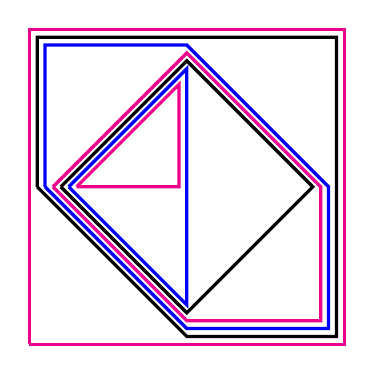
\begin{tikzpicture}[scale=2]
    \draw[magenta, very thick] (0.00,0.00)--(2.00,0.00)--(2.00,2.00)--(0.00,2.00)--(0.00,0.00);
    \draw[black,   very thick] (0.05,1.00)--(0.05,1.95)--(1.95,1.95)--(1.95,0.05)--(1.00,0.05)--(0.05,1.00);
    \draw[blue,    very thick] (0.10,1.00)--(0.10,1.90)--(1.00,1.90)--(1.90,1.00)--(1.90,0.10)--(1.00,0.10)--(0.10,1.00);
    \draw[magenta, very thick] (0.15,1.00)--(1.00,1.85)--(1.85,1.00)--(1.85,0.15)--(1.00,0.15)--(0.15,1.00);
    \draw[black,   very thick] (0.20,1.00)--(1.00,1.80)--(1.80,1.00)--(1.00,0.20)--(0.20,1.00);
    \draw[blue,    very thick] (0.25,1.00)--(1.00,1.75)--(1.00,0.25)--(0.25,1.00);
    \draw[magenta, very thick] (0.30,1.00)--(0.95,1.65)--(0.95,1.00)--(0.30,1.00);
  \end{tikzpicture}
  \caption{Seven nested convex polygons in the $3 \times 3$ grid.}
\end{figure}

\begin{question}
  If we think of each polygon having the same height, what is the greatest
  volume that we can make by stacking the polygons this way?
\end{question}

\begin{related}
  \item What is the largest sum of the perimeters? The least?
  \item What is the largest sum of the number of vertices? The least?
  \item How many ways are there to stack $n^2 - 2$ polygons like this?
    Any number of polygons?
  \item Does this generalize to polyhedra in the $n \times n \times n$ cube?
  \item Does this generalize to polygons on a triangular grid?
\end{related}
\end{document}
